\section{Dynamic Obstacles Avoidance (MPC-H)}
For the dynamic obstacles avoidance task, we have considered the same four assumptions already made for the static avoidance (as reported at the beginning of the Section \ref{chap:StaticObstacleAvoidance}) with 3 additional ones:
\begin{itemize}
    \item the dynamic obstacle has a constant speed throughout the whole scenario;
    \item the dynamic obstacle follows the same trajectory as the ego vehicle but it stays always on the right lane;
    \item the distance between two consecutive dynamic obstacles is in any case at least equal to twice the safety distance evaluated considering the speed of the ego vehicle.
\end{itemize}

Thanks to these additional assumptions, once the ego vehicle detects the obstacle in motion, it calculates the 5 zones needed to perform the overtaking maneuver correctly. As a matter of fact, we have kept the same 5 zones nearby each obstacle with some adjustments to make them work also for dynamic obstacles. 
In case a dynamic obstacle is detected, the zones are evaluated in a different way with respect to those evaluated in case of a static obstacle detection. These are the steps followed in order to calculate the 5 zones: 
\begin{enumerate}
    \item as soon as the obstacle is detected, its position and speed are acquired by the system;
    \item the trajectory of the dynamic obstacle is predicted;
    \item the safety distance is evaluated considering only the speed of the ego vehicle;
    \item Zones 1, 2 and 3 are evaluated as for the static obstacle case, but they are relative to the position of the obstacle in the future; to find the right points on the map, the following relations are used:
    \begin{equation}
        V_{relative} = V_{ref} - V_{obs}
    \end{equation}
    \begin{equation}
            DetectionTime = \frac{d-40m-SafetyDistance}{V_{relative}}
    \end{equation}
    \begin{equation}
            SafeTime = \frac{d-SafetyDistance}{V_{relative}}
    \end{equation}
    \begin{equation}
            EndTime = \frac{d+10m}{V_{relative}}
    \end{equation}
    \begin{equation}
            DetectionStep = DetectionTime/Ts
    \end{equation}
    \begin{equation}
            SafeStep = SafeTime/Ts
    \end{equation}
    \begin{equation}
            EndStep  = EndTime/Ts
    \end{equation}
    \begin{equation}
            DetIdx = ActualIdx+DetectionStep
    \end{equation}
    \begin{equation}
            SafeIdx = ActualIdx+SafeStep
    \end{equation}
    \begin{equation}
            EndIdx = ActualIdx+EndStep
    \end{equation}
    \begin{equation}
            EntryIdx = EndIdx+\frac{max(SafeDistance,40)}{V_{ref}Ts}   
    \end{equation}
    where $d$ is the distance from the obstacle when it is detected and the parameters containing $Idx$ in their name are the indexes in the reference map, corresponding to the points where the zones are defined (following the procedure described in the static obstacle section [\ref{chap:StaticObstacleAvoidance}]).
    In this case we have used indexes in the map because they are the easiest way to represent the predicted trajectory of the obstacle. However, this "trick" is only feasible in a simulation environment while in reality a different prediction algorithm is needed, but this goes beyond the purposes of our project.
    \item as shown in the previous equations, the $EntryPoint$ is no longer always placed 40 meters after the $EndPoint$, but it is chosen equal to the maximum value between the $Safety Distance$ and 40 $m$.
\end{enumerate}
Once found, these points are passed to the same constraint generator function used for the static obstacle avoidance task.

\subsection{Dynamic Obstacle Avoidance Tests}
In order to test the performance of our controller when dynamic obstacles are involved, we have set up 2 simulations exploiting the same 22 scenarios used for the Static Obstacle Avoidance tests (Section \ref{chap:static_obstacle_avoidance_tests}). Both simulations have been performed at the maximum and minimum speed of the range suitable for the MPC-H ($40\div100$  $km/h$).  

\subsubsection{Single Dynamic Obstacle}
Firstly, we have implemented a simple simulation considering a single obstacle in motion to verify the correctness of the overtaking algorithm. In particular, we have placed an obstacle with a starting position equal to the 40\% of the total length of the considered scenario with a constant speed that depends on the speed of the ego vehicle. Indeed, when the simulation is performed with 100 $km/h$ speed for the ego vehicle, the obstacle will have a constant speed of 50 $km/h$ while it will have a constant speed of 10 $km/h$ when the ego vehicle travels at 40 $km/h$. In Figure \ref{fig:single_dynamic_obstacle_avoidance} the passing maneuver performed at 100 $km/h$ is shown.

\begin{figure}[H]
\centering

    \begin{subfigure}{.33\textwidth}
    \centering
   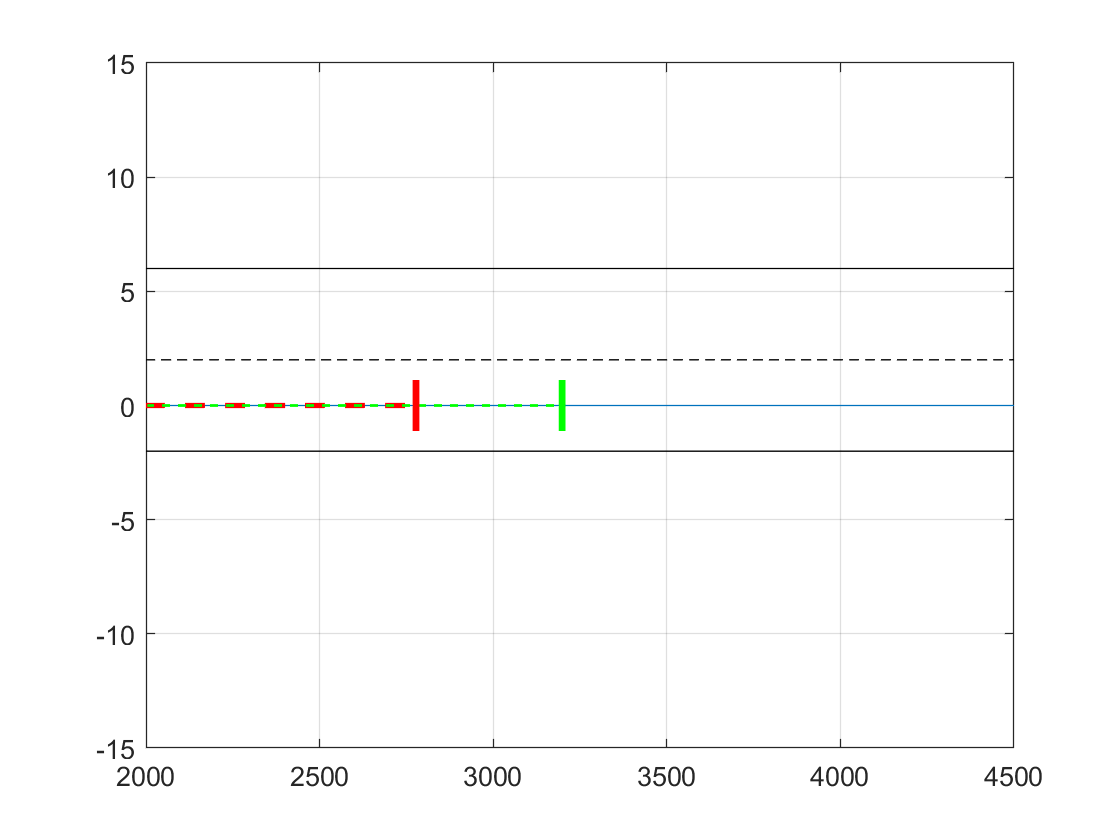
\includegraphics[width=1.1\textwidth,keepaspectratio]{Figures/overtake_single_dynamic_left.png}
    \caption{Approaching the obstacle}
    \label{subfig:single_left}
    \end{subfigure}%
    \begin{subfigure}{.33\textwidth}
    \centering
    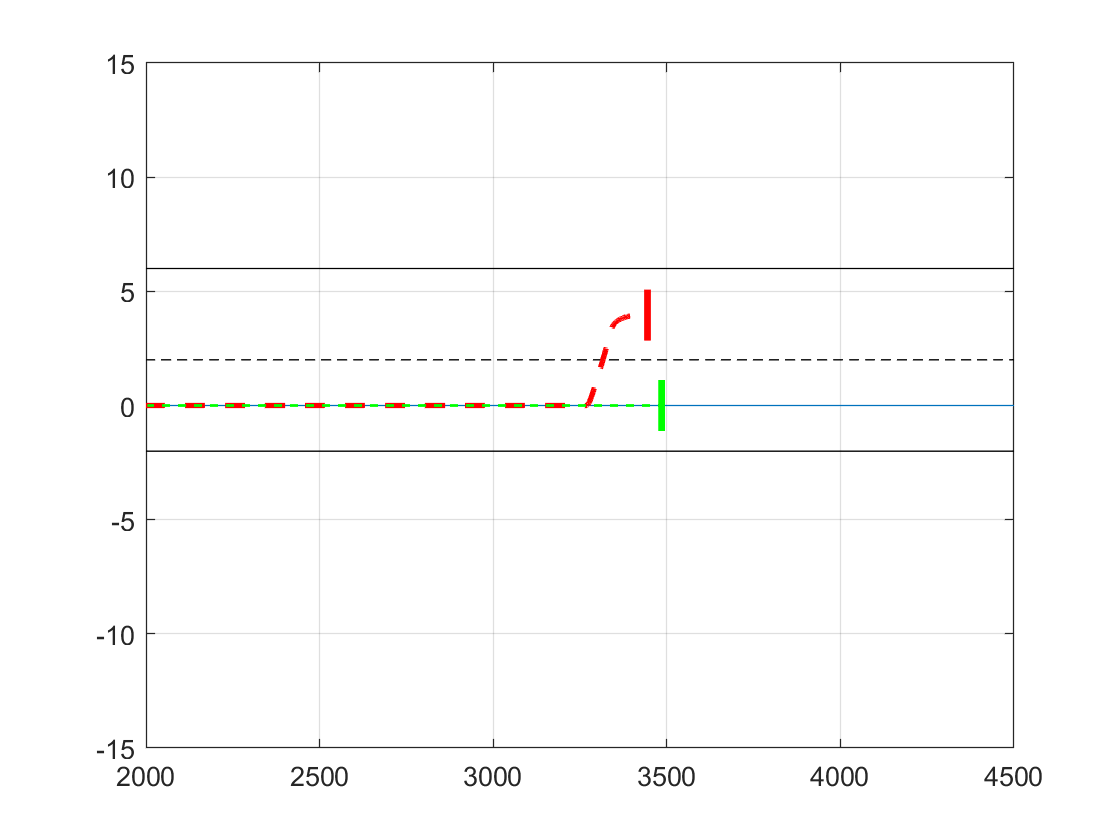
\includegraphics[width=1.1\textwidth,keepaspectratio]{Figures/overtake_single_dynamic_center.png}
    \caption{Overtaking phase}
    \label{subfig:single_center}
    \end{subfigure}
    \begin{subfigure}{.33\textwidth}
    \centering
    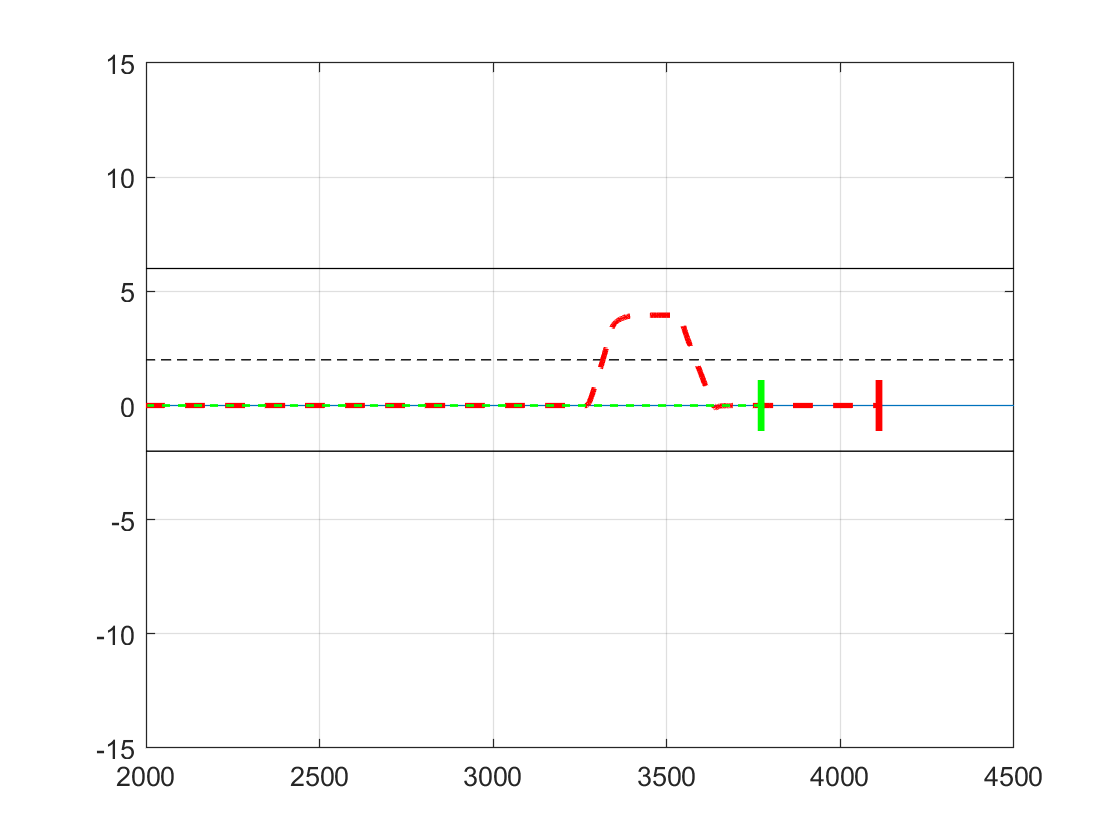
\includegraphics[width=1.1\textwidth,keepaspectratio]{Figures/overtake_single_dynamic_right.png}
    \caption{Back to the right lane}
    \label{subfig:single_right}
    \end{subfigure}
    \caption{Overtaking maneuver performed at 100 $km/h$ with an obstacle travelling at 50 $km/h$ in a straight line scenario}
    \label{fig:single_dynamic_obstacle_avoidance}
\end{figure}

Further details about the single dynamic obstacle avoidance tests performed can be found in the documents included in the repository\footnote{The ``Single\_Dynamic\_Obstacle\_Avoidance-Test\_Report" and ``Single\_Dynamic\_Obstacle\_Avoidance-Test\_Specification\_Report" files generated by Simulink Test are included in the /Documentation/Test Reports/ file path.}.\\

The tests performed have given great results at 40 $km/h$ while there have been 2 fails at 100 $km/h$. The fails have been found in the curved scenarios travelled at 100 $km/h$ in a counterclockwise direction with a curvature radius of 300 $m$ and 500 $m$. The same considerations made in Section \ref{subsection:failed_tests} and at the end of Section \ref{subsection:multiple_static} are still valid here. The problem is that, when the vehicle is at the beginning of Zone 3, the lateral deviation is not grater of or equal to 2 $m$ yet. As already said for the other fails of this kind, these can be considered as minor failures.

\subsubsection{Static and Dynamic Obstacles} 

After performing the test with a single dynamic obstacle, we have decided to integrate the dynamic obstacles avoidance algorithm with the static one, so we have built a test-bench with both static and dynamic obstacles. For this test we have considered a total of 5 obstacles (4 static and 1 dynamic) placed on the maps as follows:
\begin{itemize}
    \item Obstacle 1 (static) : placed at 7.5/100 of the total length of the map;
    \item Obstacle 2 (static) : placed at 23/100 of the total length of the map;
    \item Obstacle 3 (static) : placed at 24/100 of the total length of the map;
    \item Obstacle 4 (dynamic) : starting position at 30/100 of the total length of the map with a constant speed of 10 $km/h$;
    \item Obstacle 5 (dynamic) : starting position at 36/100 of the total length of the map with a constant speed of 20 $km/h$.
\end{itemize}

This obstacles configuration is not valid for testing purposes when considering shorter scenarios, as in the case of curved scenarios with 500 $m$ and 300 $m$ of curvature radius. In these situations, we have tuned the positioning of a total of 4 obstacles as follows:
\begin{itemize}
    \item Obstacle 1 (static) : placed at 15/100 of the total length of the map;
    \item Obstacle 2 (static) : placed at 16/100 of the total length of the map;
    \item Obstacle 3 (dynamic) : starting position at 43/100 of the total length of the map in case of 500 $m$ curvature radius and starting position at 45/100 of the total length of the map in case of 300 $m$ curvature radius (constant speed of 10 $km/h$);
    \item Obstacle 4 (dynamic) : starting position at 56/100 of the total length of the map in case of 500 $m$ curvature radius and starting position at 70/100 of the total length of the map in case of 300 $m$ curvature radius (constant speed of 20 $km/h$).
\end{itemize}
As partially explained in Section \ref{subsection:multiple_static}, we have tried to place the obstacles in such a way to test the capability of our MPC-H to lengthen the overtaking maneuver when two close consecutive obstacles are detected and to come back to the right lane after passing an obstacle in motion completing another passing maneuver after a while when detecting the next obstacle. 
\\Figure \ref{fig:static_and_dynamic_obstacle_avoidance} shows the steps of the avoidance maneuvers performed considering both static and dynamic obstacles.


\begin{figure}[H]
\centering

    \begin{subfigure}{.33\textwidth}
    \centering
   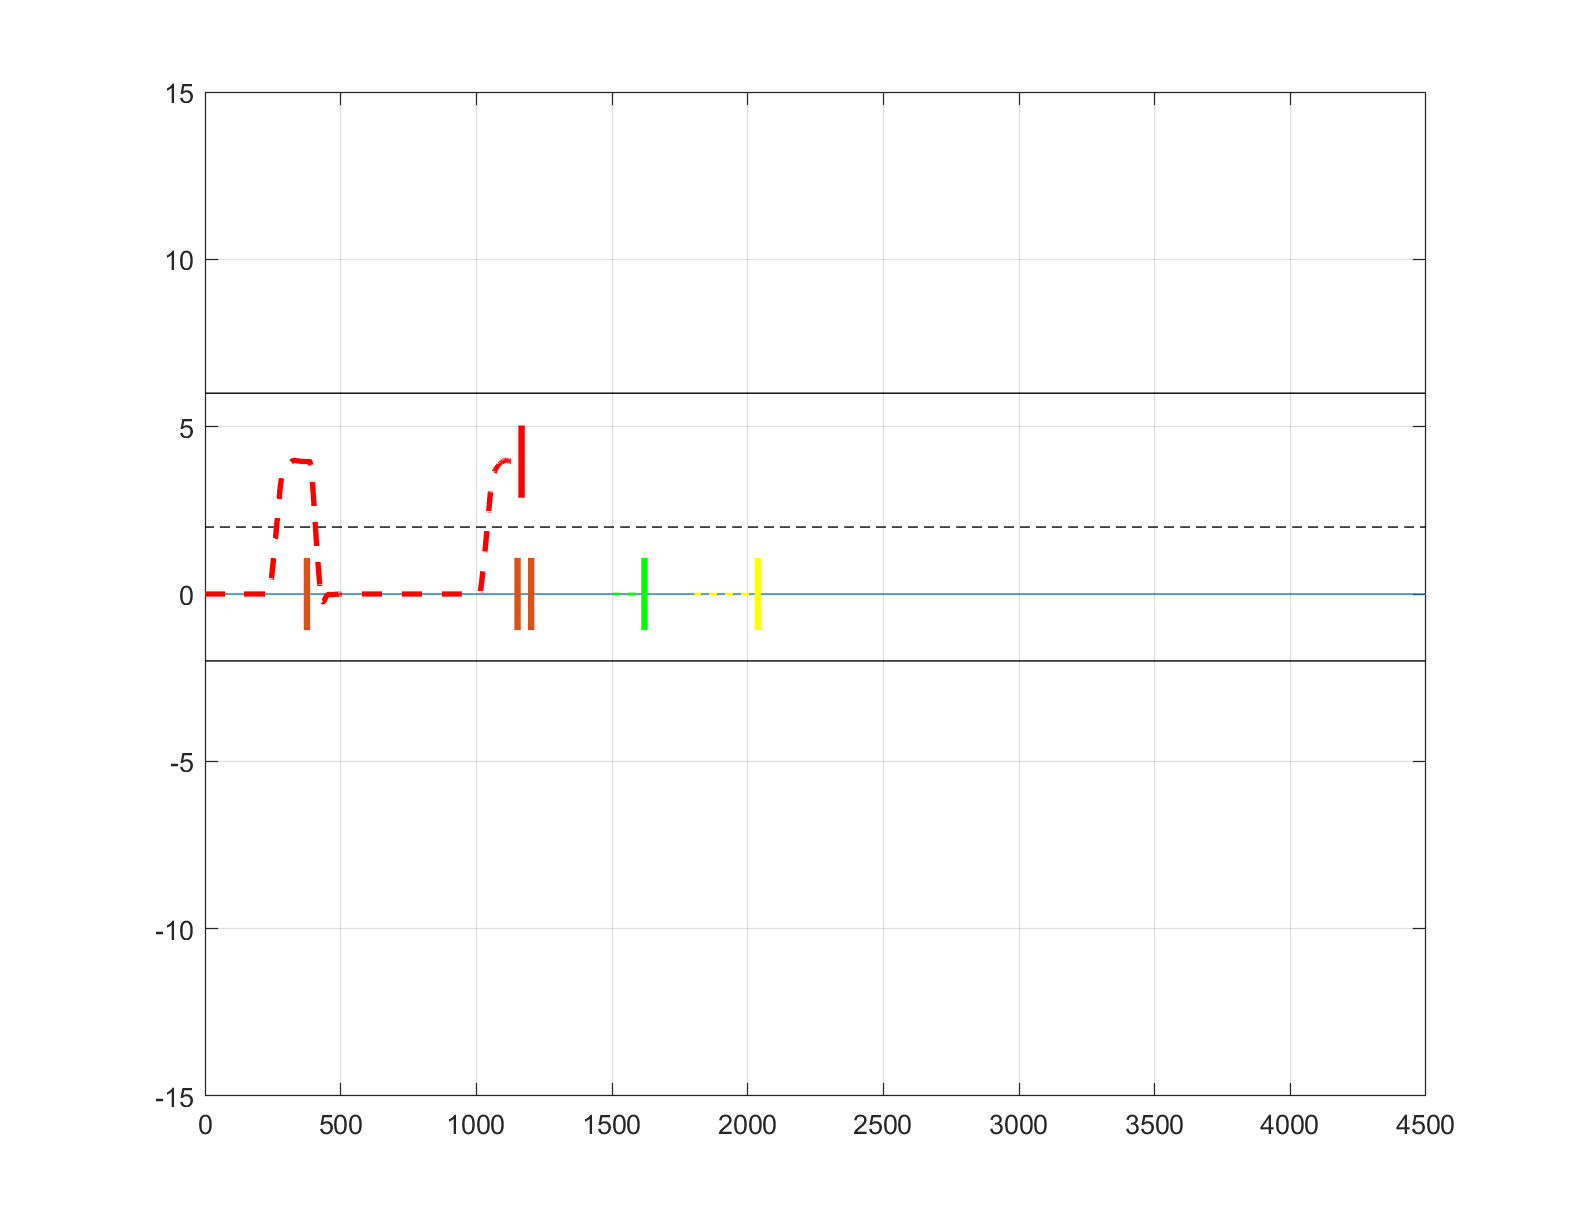
\includegraphics[width=1.1\textwidth,keepaspectratio]{Figures/overtake_multiple_left.png}
    \caption{Static obstacles}
    \label{subfig:multiple_left}
    \end{subfigure}%
    \begin{subfigure}{.33\textwidth}
    \centering
    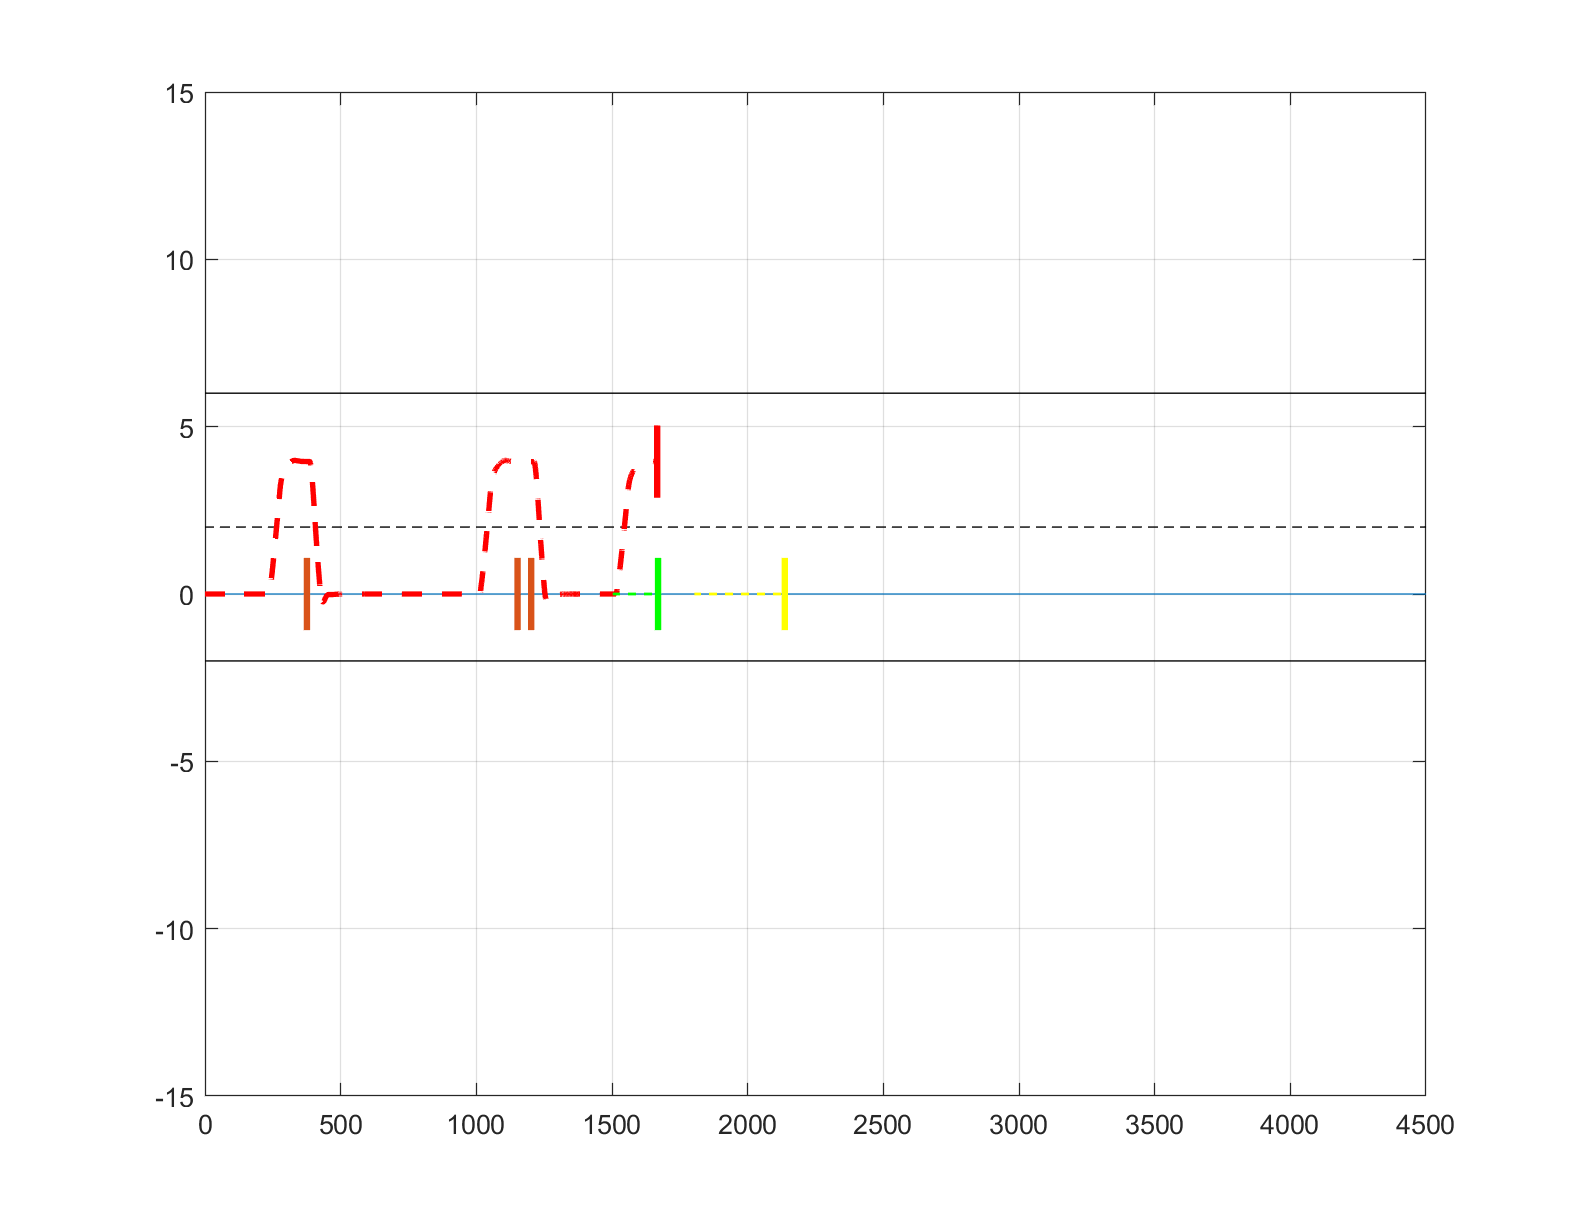
\includegraphics[width=1.1\textwidth,keepaspectratio]{Figures/overtake_multiple_center.png}
    \caption{Slower moving obstacle}
    \label{subfig:multiple_center}
    \end{subfigure}
    \begin{subfigure}{.33\textwidth}
    \centering
    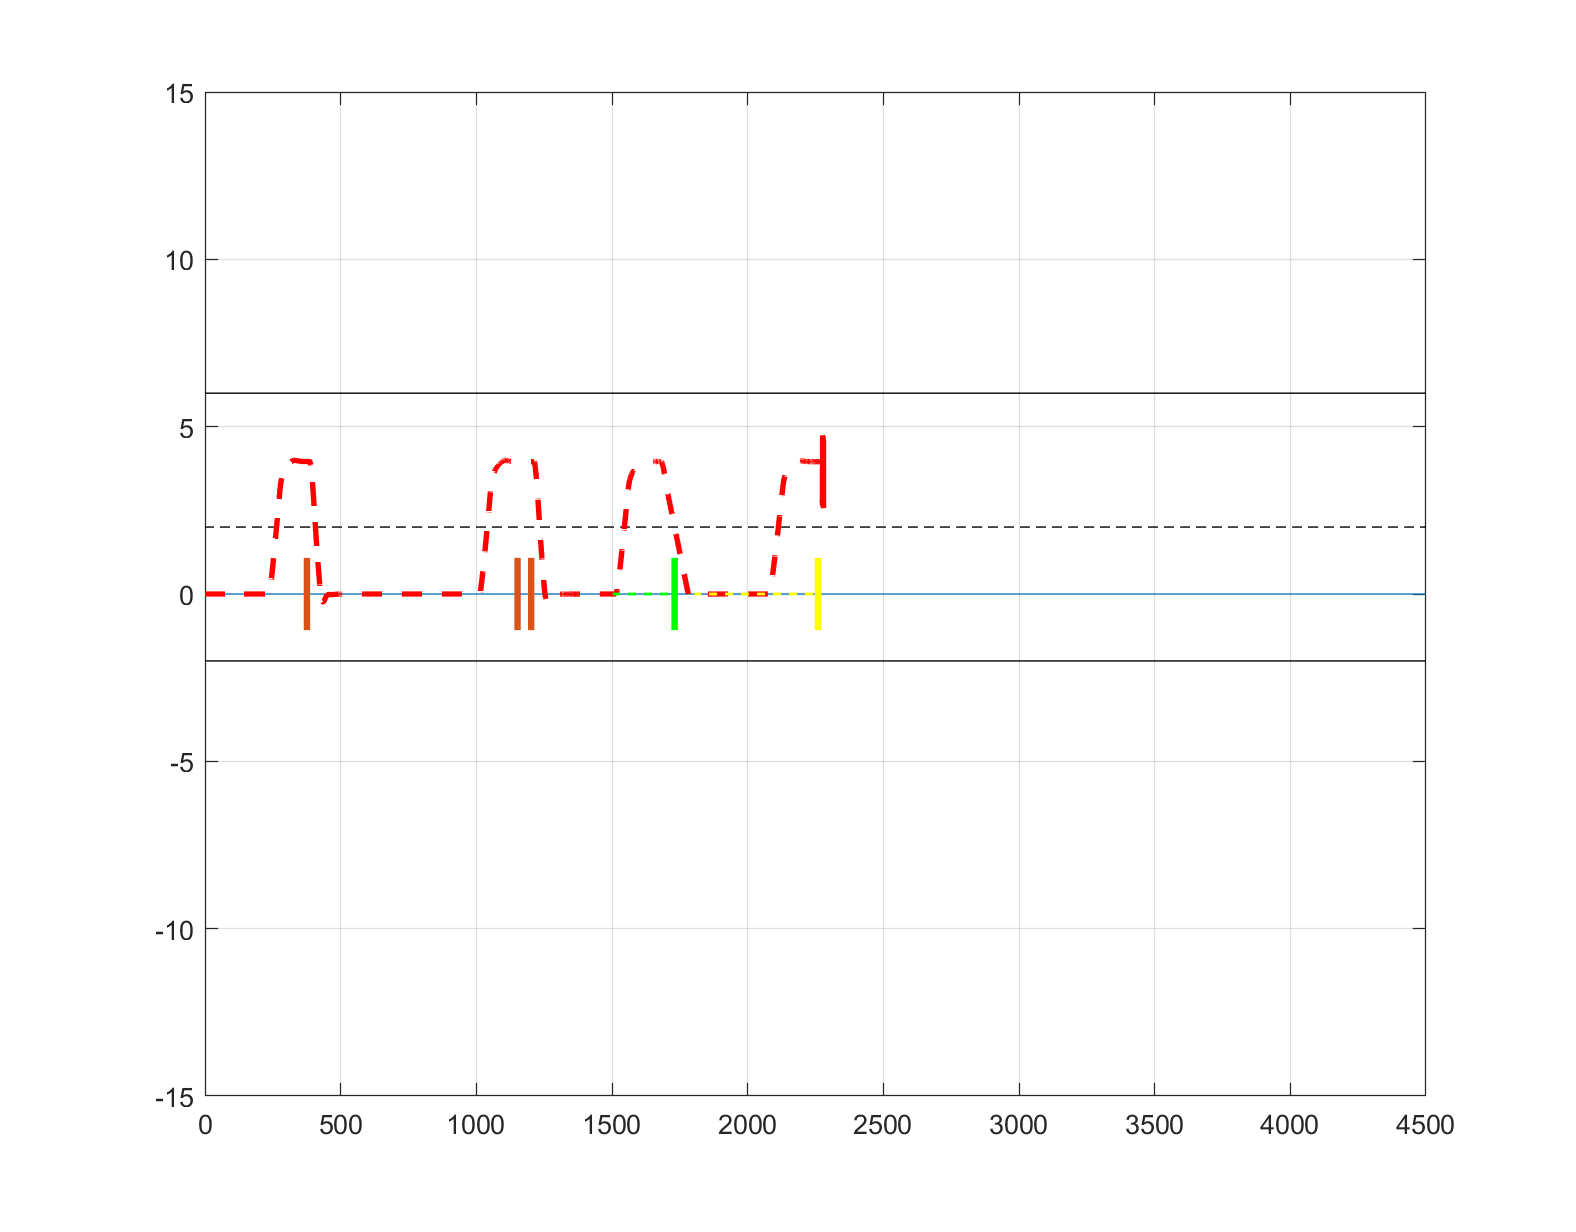
\includegraphics[width=1.1\textwidth,keepaspectratio]{Figures/overtake_multiple_right.png}
    \caption{Faster moving obstacle}
    \label{subfig:multiple_right}
    \end{subfigure}
    \caption{Overtaking maneuvers performed at 100 $km/h$ with (from left to right) three static obstacles and two dynamic obstacles travelling respectively at 10 $km/h$ (green) and 20 $km/h$ (yellow) in a straight line scenario}
    \label{fig:static_and_dynamic_obstacle_avoidance}
\end{figure}

Further details about the tests performed can be found in the documents included in the repository\footnote{The ``Dynamic\_and\_static\_obstacle\_avoidance-test\_report" and ``Dynamic\_and\_static\_obstacle\_avoi-dance-test\_specification\_report" files generated by Simulink Test are included in the /Documentation/Test Reports/ file path.}.\\
Again the only failure of the test is the one corresponding to the curved scenario with a curvature radius of 300 $m$ when the ego-vehicle is travelling at 100 $km/h$ counterclockwise.







